% +------------------------------------------------------------------------+
% | CGAL Reference Manual:  hds.tex
% +------------------------------------------------------------------------+
% | Combinatoric and geometry of polyhedral surfaces in 
% | halfedge representation.
% |
% | 11.10.1996   Lutz Kettner
% |              Start rewriting the whole stuff
% | 
\RCSdef{\hdsRev}{$Revision$}
\RCSdefDate{\hdsDate}{$Date$}
% +------------------------------------------------------------------------+

\ccParDims

\chapter{Halfedge Data Structures}
\label{chapterHalfedgeDS}
\ccChapterRelease{\hdsRev. \ \hdsDate}\\
\ccChapterAuthor{Lutz Kettner}

\minitoc

% +------------------------------------------------------------------------+
\section{Release Note}

Beginning with \cgal\ R2.3, this package has a new design.  The old
design is still available for backwards compatibility and to support
older compiler, such as MSVC++6.0. However its use is deprecated and
the manual pages are not converted into this new manual
format. Instead, see its old documentation in the manual of 
deprecated packages. The two designs are not interchangeable.

% +------------------------------------------------------------------------+
\section{Introduction}

A halfedge data structure (abbreviated as \ccc{HalfedgeDS}, or
\ccc{HDS} for template parameters) is an edge-centered data structure
capable of maintaining incidence informations of vertices, edges and
faces, for example for planar maps, polyhedra, or other orientable,
two-dimensional surfaces embedded in arbitrary dimension. Each edge is
decomposed into two halfedges with opposite orientations. One incident
face and one incident vertex are stored in each halfedge.  For each
face and each vertex, one incident halfedge is stored.  Reduced
variants of the halfedge data structure can omit some of these
informations, for example the halfedge pointers in faces or the
storage of faces at all.

\begin{ccTexOnly}
    \vspace{-4mm}
    \begin{center}
      \parbox{0.4\textwidth}{%
          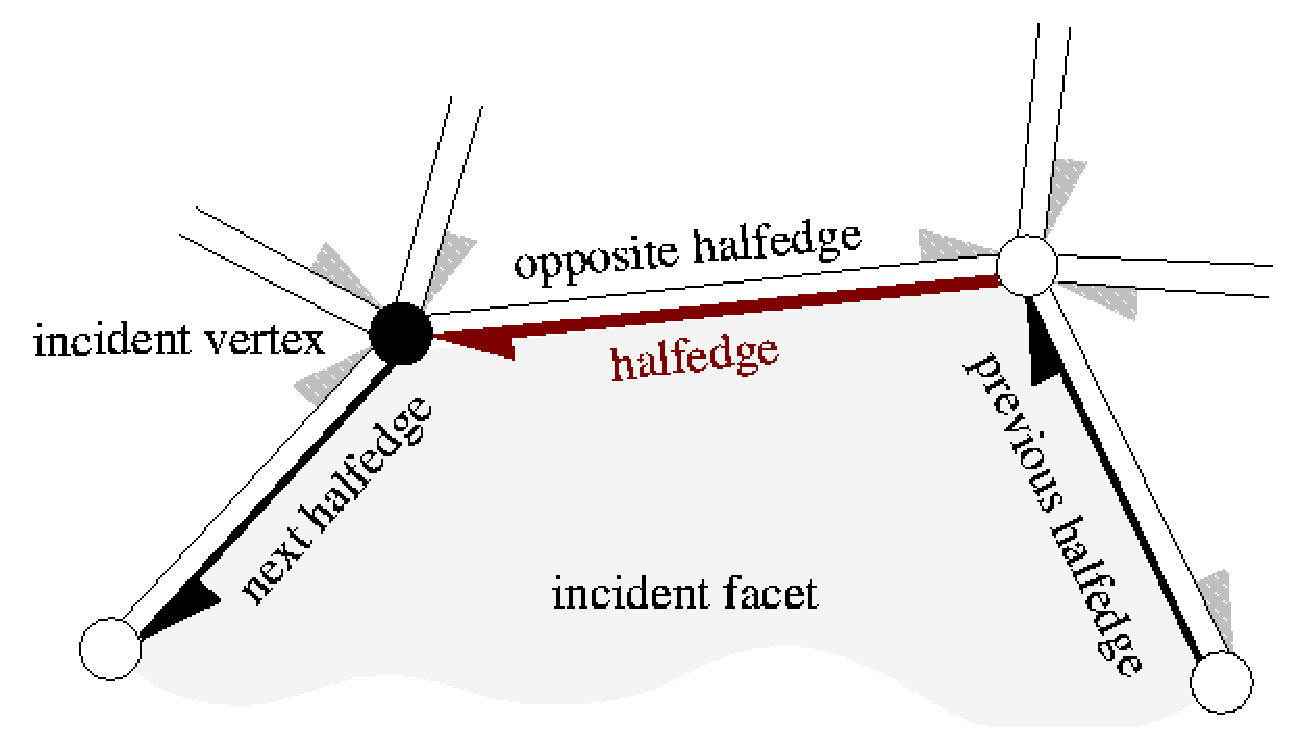
\includegraphics[width=0.4\textwidth]{fig/halfedge.ips}%
      }
    \end{center}
    \vspace{-3mm}
\end{ccTexOnly}

\begin{ccHtmlOnly}
    <CENTER>
    <A HREF="./halfedge.gif">
        <img src="./halfedge_small.gif" alt="Halfedge Diagram"></A><P>
    </CENTER>
\end{ccHtmlOnly}

The halfedge data structure is a combinatorial data structure,
geometric interpretation is added by classes built on top of the
halfedge data structure.  These classes might be more convenient to
use than the halfedge data structure directly, since the halfedge data
structure is meant as an implementation layer.  See for example the
\ccc{CGAL::Polyhedron_3} class in Chapter~\ref{chapterPolyhedron}.

The data structure provided here is also known as the
FE-structure~\cite{w-ebdss-85}, as
halfedges~\cite{m-ism-88,bfh-mgedm-95} or as the doubly connected edge
list (DCEL)~\cite{bkos-cgaa-97}, although the original reference for
the DCEL~\cite{mp-fitcp-78} describes a different data structure. The
halfedge data structure can also be seen as one of the variants of the
quad-edge data structure~\cite{gs-pmgsc-85}. In general, the quad-edge
data can represent non-orientable 2-manifolds, but the variant here is
restricted to orientable 2-manifolds only. An overview and comparison
of these different data structures together with a thorough
description of the design implemented here can be found
in~\cite{k-ugpdd-99}.  

The design presented here is a revised and incompatible version of the
previous design~\cite{k-ddsps-98} as used in \cgal\ R2.2 and earlier
releases. Files and identifier names are disjoint with the old design
which allows for both versions to co-exists. However, classes using a
halfedge data structure can only use one design. For example the
polyhedral surface \ccc{Polyhedron_3} uses by default the new
design. See Chapter~\ref{chapterPolyhedron} for how to still select
the old implementation.

% +------------------------------------------------------------------------+
\section{Software Design}


\begin{ccTexOnly}
  \begin{figure}
    \begin{center}
      \parbox{0.7\textwidth}{%
          \includegraphics[width=0.7\textwidth]{fig/hds_design.ips}%
      }
    \end{center}
    \caption{Responsibilities of the different layers in the 
             halfedge data-structure design.}
    \label{figureHalfedgeDSDesign}
  \end{figure}
\end{ccTexOnly}

\begin{ccHtmlOnly}
    <CENTER>
    <A NAME="figureHalfedgeDSDesign">
        <img src="./hds_design_col.gif"
         alt="Halfedge Data-Structure Design"><BR>
    Figure: Responsibilities of the different layers in the 
            halfedge data-structure design.
    <P>
    </CENTER>
\end{ccHtmlOnly}

Figure~\ccTexHtml{\ref{figureHalfedgeDSDesign}}{}\begin{ccHtmlOnly}
  <A HREF="Chapter_main.html#figureHalfedgeDSDesign"><IMG 
  SRC="cc_ref_up_arrow.gif" ALT="reference arrow" WIDTH="10" HEIGHT="10"></A>
\end{ccHtmlOnly}
illustrates the responsibilities of the three layers of the software
design, with the \ccc{CGAL::Polyhedron_3} as an example for the top
layer.  The items provide the space for the information that is
actually stored, i.e., with member variables and access member
functions in \ccc{Vertex}, \ccc{Halfedge}, and \ccc{Face}
respectively. Halfedges are required to provide a reference to the
next halfedge and to the opposite halfedge.  Optionally they may
provide a reference to the previous halfedge, to the incident vertex,
and to the incident face. Vertices and faces may be empty. Optionally
they may provide a reference to the incident halfedge. The options
mentioned are supported in the halfedge data structure and the
polyhedron, for example, Euler operations update the optional
references if they are present. Furthermore, the item classes can be
extended with arbitrary attributes and member functions, which will be
promoted by inheritance to the actual classes used for the polyhedron.

Vertices, halfedges, and faces are passed as local types of the
\ccc{Items} class to the halfedge data structure and polyhedron.
Implementations for vertices, halfedges and faces are provided that
fulfill the mandatory part of the requirements. They can be used as
base classes for extensions by the user. Richer implementations are
also provided to serve as defaults; for polyhedra they provide all
optional incidences, a three-dimensional point in the vertex type and
a plane equation in the face type.

The \ccc{Halfedge_data_structure}, concept \ccc{HalfedgeDS}, is
responsible for the storage organization of the items. Currently,
implementations using internally a bidirectional list or a
vector are provided. The \ccc{HalfedgeDS} defines the handles and iterators
belonging to the items. These types are promoted to the declaration of
the items themselves and are used there to provide the references to
the incident items. This promotion of types is done with a template
parameter \ccc{Refs} of the item types.  The halfedge data structure
provides member functions to insert and delete items, to traverse all
items, and it gives access to the items.

There are two different models for the \ccc{HalfedgeDS} concept available,
\ccc{HalfedgeDS_list} and \ccc{HalfedgeDS_vector}, and more might come.
Therefore we have kept their interface small and factored out common
functionality into separate helper classes, \ccc{HalfedgeDS_decorator},
\ccc{HalfedgeDS_const_decorator}, and \ccc{HalfedgeDS_items_decorator},
which are not shown in
Figure~\ccTexHtml{\ref{figureHalfedgeDSDesign}}{}\begin{ccHtmlOnly} <A
HREF="Chapter_main.html#figureHalfedgeDSDesign"><IMG
SRC="cc_ref_up_arrow.gif" ALT="reference arrow" WIDTH="10"
HEIGHT="10"></A>
\end{ccHtmlOnly}, but would be placed at the side of the \ccc{HalfedgeDS}
since they broaden that interface but do not hide it.  These helper
classes contain operations that are useful to implement the operations
in the next layer, for example, the polyhedron. They add, for example,
the Euler operations and partial operations from which further Euler
operations can be built, such as inserting an edge into the ring of
edges at a vertex.  Furthermore, the helper classes contain adaptive
functionality.  For example, if the \ccc{prev()} member function is
not provided for halfedges, the \ccc{find_prev()} member function of
a helper class searches in the positive direction along the face for
the previous halfedge. But if the \ccc{prev()} member function is
provided, the \ccc{find_prev()} member function simply calls it. This
distinction is resolved at compile time with a technique called {\em
compile-time tags}, similar to iterator tags in~\cite{sl-stl-95}.

The \ccc{Polyhedron_3} as an example for the third layer adds the
geometric interpretation, provides an easy-to-use interface of
high-level functions, and unifies the access to the flexibility
provided underneath.  It renames face to facet, which is more common
for three-dimensional surfaces.  The interface is designed to protect
the integrity of the internal representation, the handles stored in
the items can no longer directly be written by the user.  The
polyhedron adds the convenient and efficient circulators, see the
Support Library Manuals, for accessing the circular sequence of edges
around a vertex or around a facet. To achieve this, the
\ccc{Polyhedron_3} derives new vertices, halfedges and facets from those
provided in \ccc{Items}.  These new items are those actually used in
the \ccc{HalfedgeDS}, which gives us the coherent type
structure in this design, especially if compared to our previous
design.


% +========================================================================+
\section{Example Programs}
% +========================================================================+
\label{sectionHdsExamples}


% +-------------------------------------------------------------+
\subsection{The Default Halfedge Data Structure}

The following example program uses the default halfedge data structure
and the decorator class. The default halfedge data structure uses a
list-based representation. All incidences of the items and a point
type for vertices are defined. The trivial traits class provides the
type used for the point. The program creates a loop, consisting
of two halfedges, one vertex and two faces, and checks its validity.

\begin{ccTexOnly}
    \vspace{-4mm}
    \begin{center}
      \parbox{0.3\textwidth}{%
          \includegraphics[width=0.3\textwidth]{fig/loop.ips}%
      }
    \end{center}
    \vspace{-3mm}
\end{ccTexOnly}

\begin{ccHtmlOnly}
    <CENTER>
      <img src="./loop.gif" alt="Loop Example"><P>
    </CENTER>
\end{ccHtmlOnly}

\ccIncludeExampleCode{HalfedgeDS/hds_prog_default.C}


% +-------------------------------------------------------------+
\subsection{A Minimal Halfedge Data Structure}

The following program defines a minimal halfedge data structure using
the minimal items class \ccc{CGAL::HalfedgeDS_min_items} and a
list-based halfedge data structure. The result is a data structure
maintaining only halfedges with next and opposite pointers.  No
vertices or faces are stored. The data structure represents an {\em
  undirected graph}.

\ccIncludeExampleCode{HalfedgeDS/hds_prog_graph.C}


% +-------------------------------------------------------------+
\subsection{The Default with a Vector Instead of a List}

The default halfedge data structure uses a list internally and the
maximal base classes. We change the list to a vector representation
here. Again, a trivial traits class provides the type used for the
point.  Note that for the vector storage the size of the halfedge data
structure should be reserved beforehand, either with the constructor
as shown in the example or with the \ccc{reserve()} member function.
One can later resize the data structure with further calls to the
\ccc{reserve()} member function, but only if the data structure is 
in a consistent, i.e., {\em valid}, state.

Unfortunately this example has also to expose the workaround necessary
for compilers that do not support templates as template parameters.
The workaround is necessary if the symbolic constant
\verb|CGAL_CFG_NO_TMPL_IN_TMPL_PARAM| is set. It uses a member 
template instead of the class template.

\ccIncludeExampleCode{HalfedgeDS/hds_prog_vector.C}


% +-------------------------------------------------------------+
\subsection{Example Adding Color to Faces}

This example re-uses the base class available for faces and adds a
member variable \ccc{color}.

\ccIncludeExampleCode{HalfedgeDS/hds_prog_color.C}

% +-------------------------------------------------------------+
\subsection{Example Defining a More Compact Halfedge}

\begin{ccAdvanced}
  
The halfedge data structure as presented here is slightly less space
efficient as, for example, the winged-edge data
structure~\cite{b-prcv-75}, the DCEL~\cite{mp-fitcp-78} or variants of
the quad-edge data structure~\cite{gs-pmgsc-85}.  On the other hand,
it does not require any search operations during traversals. A
comparison can be found in~\cite{k-ugpdd-99}.

The following example trades traversal time for a compact storage
representation using traditional C techniques (i.e., type casting and
the assumption that pointers, especially those from {\tt malloc} or
{\tt new}, point to even addresses). The idea goes as follows: The
halfedge data structure allocates halfedges pairwise.  Concerning the
vector-based data structure this implies that the absolute value of
the difference between a halfedge and its opposite halfedge is always
one with respect to C pointer arithmetic. We can replace the opposite
pointer by a single bit encoding the sign of this difference.  We will
store this bit as the least significant bit in the next halfedge
handle.  Furthermore, we do not implement a pointer to the previous
halfedge. What remains are three pointers per halfedge. 

We use the static member function \ccc{halfedge_handle()} to convert
from pointers to halfedge handles. The same solution can be applied to
the list-based halfedge data structure \ccc{CGAL::HalfedgeDS_list},
see \texttt{examples/HalfedgeDS/hds\_prog\_compact2.C}. Here is the
example for the vector-based data structure.

\ccIncludeExampleCode{HalfedgeDS/hds_prog_compact.C}

\end{ccAdvanced}

% +-------------------------------------------------------------+
\subsection{Example Using the Halfedge Iterator}

Two edges are created in the default halfedge data structure.
The halfedge iterator is used to count the halfedges.
%\newpage

\ccIncludeExampleCode{HalfedgeDS/hds_prog_halfedge_iterator.C}

% +-------------------------------------------------------------+
\subsection{Example for an Adapter to Build an Edge Iterator}

Three edges are created in the default halfedge data structure.
The adapter \ccc{N_step_adaptor} is used to declare the edge
iterator used in counting the edges.

\ccIncludeExampleCode{HalfedgeDS/hds_prog_edge_iterator.C}

% +--------------------------------------------------------+

%% % =============================================================================
% The CGAL Reference Manual
% Chapter: Geometric Optimisation
% -----------------------------------------------------------------------------
% file   : doc_tex/basic/Optimisation/Optimisation_ref/main.tex
% package: Optimisation_doc
% author : Sven Sch�nherr <sven@inf.ethz.ch>
% -----------------------------------------------------------------------------
% $Revision$
% $Date$
% =============================================================================

\section{Reference Pages}

% =============================================================================
% The CGAL Reference Manual
% Chapter: Geometric Optimisation
% -----------------------------------------------------------------------------
% file   : doc_tex/basic/Optimisation/Optimisation_ref/reference_part.tex
% package: Optimisation_doc
% author : Sven Sch�nherr <sven@inf.ethz.ch>
% -----------------------------------------------------------------------------
% $Revision$
% $Date$
% =============================================================================

\newcommand{\inputOpt}[1]{\input{Optimisation_ref/#1.tex}}

\newcommand{\linebreakByHand}{\ccTexHtml{\linebreak[4]}{}}
\newcommand{  \newlineByHand}{\ccTexHtml{\\}{}}

% cross references
\index{minimum enclosing|see{{smallest enclosing}}}
\index{minimum spanning|see{{smallest enclosing}}}
\index{concentric spheres|see{{annulus}}}

% -----------------------------------------------------------------------------
\section*{Introduction}

This chapter describes concepts, classes, and functions for solving
geometric optimisation problems. They are divided into four categories.

\paragraph{Bounding Areas and Volumes.}
Smallest enclosing circle and ellipse (2D), smallest enclosing rectangle,
parallelogram, and strip (2D), rectangular $p$-center (2D), smallest
enclosing sphere and annulus (dD).

\paragraph{Inscribed Areas.}
Maximum area and perimeter inscribed $k$-gon (2D), extremal inscribed
$k$-gon (2D).

\paragraph{Optimal Distances.}
All furthest neigbors (2D), width of point set (3D), polytope distance (dD).

\paragraph{Advanced Techniques.}
Monotone and sorted matrix search.

\section*{Assertions}
The optimisation code uses infix \ccc{OPTIMISATION} in the assertions,
e.g.\ defining the compiler flag
\ccc{CGAL_OPTIMISATION_NO_PRECONDITIONS} switches precondition
checking off, cf.~\cgalReferToAssertions


% -----------------------------------------------------------------------------
\subsection*{Bounding Areas and Volumes}

\ccRefIdfierPage{CGAL::Min_circle_2<Traits>}\\[1ex]
\ccRefIdfierPage{CGAL::Min_circle_2_traits_2<K>}\\[1ex]
\ccRefConceptPage{MinCircle2Traits}

\smallskip

\ccRefIdfierPage{CGAL::Min_ellipse_2<Traits>}\\[1ex]
\ccRefIdfierPage{CGAL::Min_ellipse_2_traits_2<K>}\\[1ex]
\ccRefConceptPage{MinEllipse2Traits}

\smallskip

\ccRefIdfierPage{CGAL::min_rectangle_2}\\
\ccRefIdfierPage{CGAL::min_parallelogram_2}\\
\ccRefIdfierPage{CGAL::min_strip_2}\\[1ex]
\ccRefIdfierPage{CGAL::Min_quadrilateral_default_traits_2<R>}\\[1ex]
\ccRefConceptPage{MinQuadrilateralTraits_2}

\smallskip

\ccRefIdfierPage{CGAL::rectangular_p_center_2}\\[1ex]
\ccRefIdfierPage{CGAL::Rectangular_p_center_default_traits_2<R>}\\[1ex]
\ccRefConceptPage{RectangularPCenterTraits_2}

\bigskip

\ccRefIdfierPage{CGAL::Min_sphere_d<Traits>}\\
\ccRefIdfierPage{CGAL::Min_annulus_d<Traits>}\\[1ex]
\ccRefIdfierPage{CGAL::Optimisation_d_traits_2<K,ET,NT>}\\
\ccRefIdfierPage{CGAL::Optimisation_d_traits_3<K,ET,NT>}\\
\ccRefIdfierPage{CGAL::Optimisation_d_traits_d<K,ET,NT>}\\[1ex]
\ccRefConceptPage{OptimisationDTraits}

% -----------------------------------------------------------------------------
\subsection*{Inscribed Areas}

\ccRefIdfierPage{CGAL::maximum_area_inscribed_k_gon_2}\\
\ccRefIdfierPage{CGAL::maximum_perimeter_inscribed_k_gon_2}\\
\ccRefIdfierPage{CGAL::extremal_polygon_2}\\[1ex]
\ccRefIdfierPage{CGAL::Extremal_polygon_area_traits_2<K>}\\
\ccRefIdfierPage{CGAL::Extremal_polygon_perimeter_traits_2<K>}\\[1ex]
\ccRefConceptPage{ExtremalPolygonTraits_2}

% -----------------------------------------------------------------------------
\subsection*{Optimal Distances}

%\ccRefIdfierPage{CGAL::width_2}%\\[1ex]
%\ccRefIdfierPage{CGAL::Min_quadrilateral_default_traits_2<K>}\\[1ex]
%\ccRefConceptPage{MinQuadrilateralTraits_2}

%\smallskip

\ccRefIdfierPage{CGAL::all_furthest_neighbors_2}\\[1ex]
%\ccRefIdfierPage{CGAL::All_furthest_neighbors_default_traits_2<R>}\\[1ex]
\ccRefConceptPage{AllFurthestNeighborsTraits_2}

\smallskip

\ccRefIdfierPage{CGAL::Width_3<Traits>}\\[1ex]
\ccRefIdfierPage{CGAL::Width_default_traits_3<K>}\\[1ex]
\ccRefConceptPage{WidthTraits_3}

\smallskip

\ccRefIdfierPage{CGAL::Polytope_distance_d<Traits>}\\[1ex]
\ccRefIdfierPage{CGAL::Optimisation_d_traits_2<K,ET,NT>}\\
\ccRefIdfierPage{CGAL::Optimisation_d_traits_3<K,ET,NT>}\\
\ccRefIdfierPage{CGAL::Optimisation_d_traits_d<K,ET,NT>}\\[1ex]
\ccRefConceptPage{OptimisationDTraits}

% -----------------------------------------------------------------------------
\subsection*{Advanced Techniques}

\ccRefIdfierPage{CGAL::monotone_matrix_search}\\[1ex]
\ccRefIdfierPage{CGAL::Dynamic_matrix<M>}\\[1ex]
\ccRefConceptPage{MonotoneMatrixSearchTraits}\\
\ccRefConceptPage{BasicMatrix}

\smallskip

\ccRefIdfierPage{CGAL::sorted_matrix_search}\\[1ex]
\ccRefIdfierPage{CGAL::Sorted_matrix_search_traits_adaptor<F,M>}\\[1ex]
\ccRefConceptPage{SortedMatrixSearchTraits}

\smallskip

% =============================================================================

% Bounding Areas and Volumes

\inputOpt{main_Min_circle_2}
\inputOpt{main_Min_ellipse_2}
\inputOpt{main_Min_quadrilateral_2}
\inputOpt{main_Rectangular_p_centers}

\inputOpt{main_Min_sphere_d}
\inputOpt{main_Min_annulus_d}
\inputOpt{main_Optimisation_d_traits}

% Inscribed Areas

\inputOpt{main_Extremal_polygons}

% Optimal Distances

\inputOpt{main_All_furthest_neighbors}

\inputOpt{main_Width_3}

\inputOpt{main_Polytope_distance_d}


% Advanced Techniques

\inputOpt{main_Matrix_search}


% ===== EOF ===================================================================


% ===== EOF ===================================================================


% EOF
